\section{Overview}
\label{section:overview}
\col{Outline for overview:
\begin{enumerate}[(1)]
\item Reducing local distortion
\item Enhancing local relationships
\item Workflow
\end{enumerate}
}
In this work, we propose to steer high-dimensional data exploration via local data analysis. We facilitate local analysis by reducing local projection distortions. In this section, we first clarify the concept of local distortion reduction. Then we demonstrate how it supports an efficient data exploration. At last, we give an overview of the interactive exploration process supported by our method.

\subsection{Local Distortion Reduction}
Distortion usually refers to the gap between original data distances and the projected distances. We call it the \emph{distance distortion}. Our approach helps to reduce such distortions locally for a more faith perception. However, it may not be enough to support data feature analyses. There have been lots of dimension reduction techniques~\cite{jolliffe2002principal}~\cite{borg2005modern}~\cite{tenenbaum2000global}~\cite{roweis2000nonlinear}, aiming to reduce distance distortions globally. But a more recent research~\cite{DBLP:journals/tvcg/EtemadpourMPMOL15} has shown that, those projections cannot guarantee a good performance for certain analytic tasks. The main cause, in our opinion, is the existence of relationship distortions.

By 'relationship', we refer to a relative concept of distance, i.e. 'close' or 'far'. In the high-dimensional space, relationship should be defined in a certain data range and dimensional subspace. Assume that there are four data items distributed in a two-dimensional plane, as shown in Figure 2. \col{(Figure to be added.)} When talking about data A, B and C, we can say that 'C is far away from B (compared to A)'. But when talking about data B, C and D, C seems close to B (compared to D). On the other hand, C is closer to B than A in dimension X, while the opposite happens in dimension Y. When combing all data and dimensions, weaker relationships give way to the stronger ones. The weak ones (e.g. C is closer to B than A) can no longer be perceived. Even the strong ones are not as obvious as in the original context. We call it the \emph{relationship distortion}. The situation is alike in more complex real-world datasets. Integrated measurements cannot reflect local relationships precisely. That's why approximating the overall distances cannot guarantee enhanced data features.

In contrast, reducing distortion of the interested relationship can support a more targeted analysis. For example, when we talk about two objects being similar, we tend to ignore their differences temporally and vice versa. We believe that distortion reduction should be built upon certain analytic targets, namely the local data and relationships. It is the key to revealing hidden local features. That's the reason we provide two different types of distortion reduction, for different purposes. In fact, we will prove that distance distortion is a special case of relationship distortion. Both goals can actually be achieved in the same framework.\note{ Specifically, we allow users to focus on a data subset to accommodate relationships in different ranges. In addition, projection pursuit is applied to enhance relationships in different subspaces.} More details will be introduced in Section~\ref{section:method}.

\ifx
\begin{figure*}[htb]
\centering
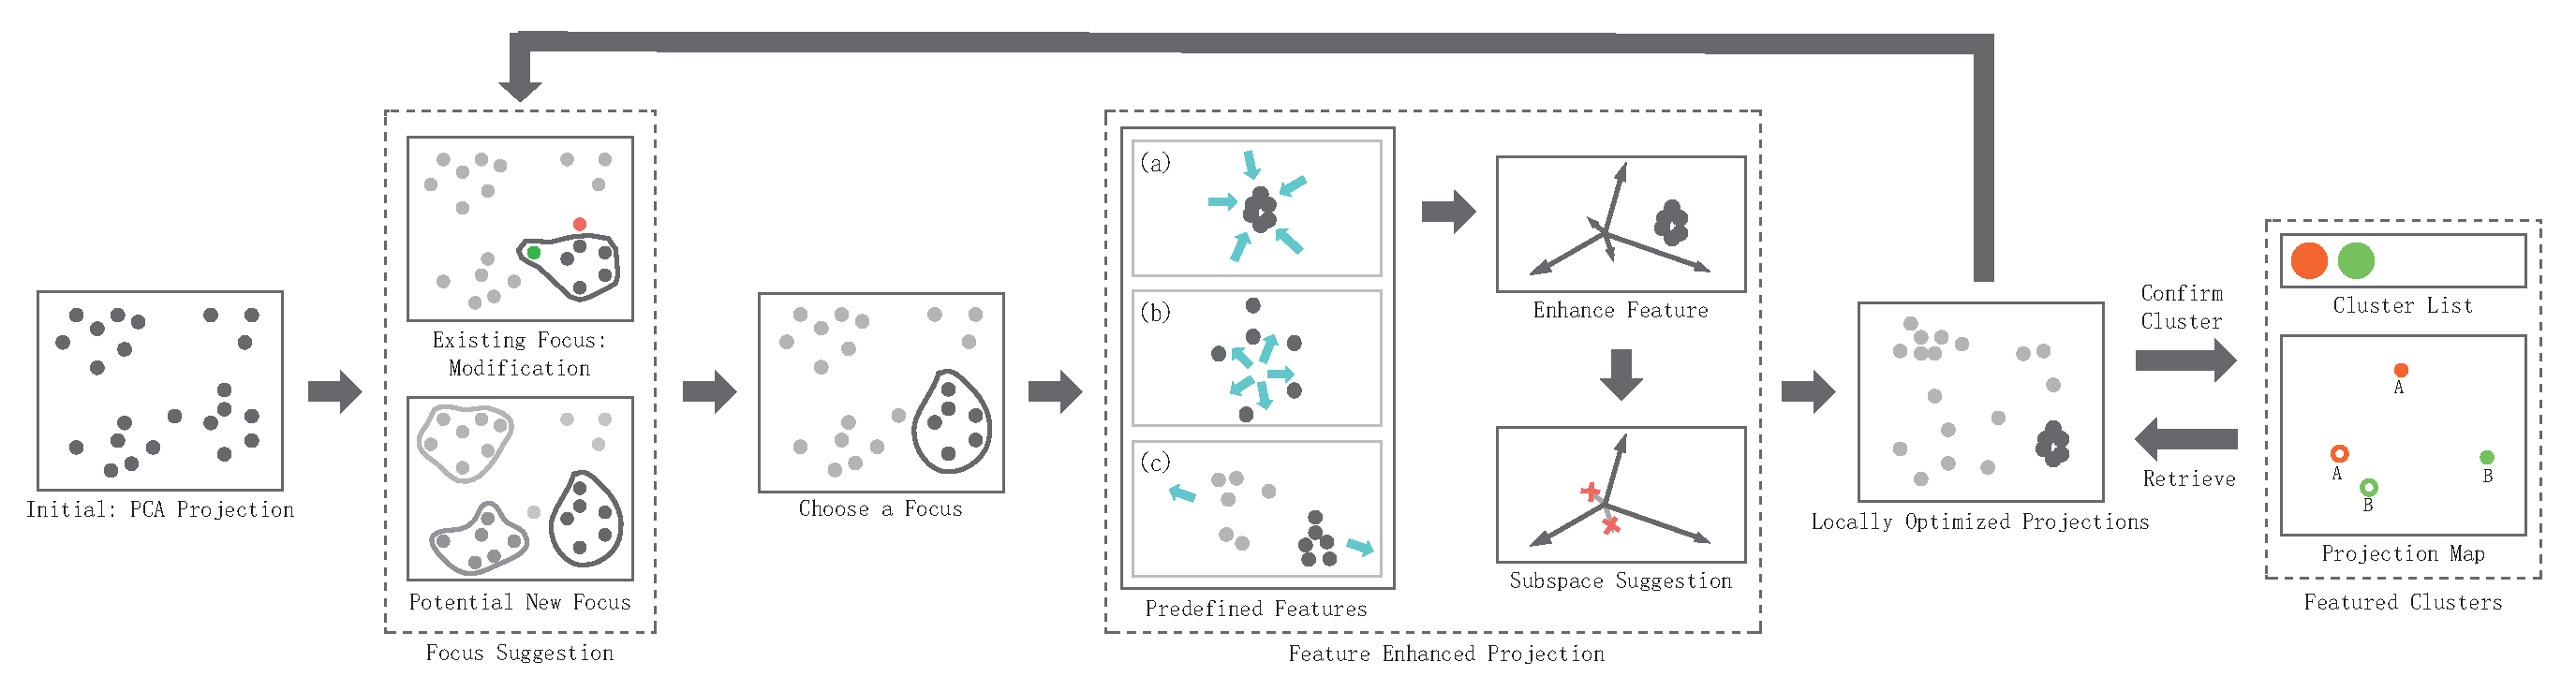
\includegraphics{images/Pipeline.eps}
\caption{Sample illustration.}
\end{figure*}
\else
\begin{figure*}[htbp]
\centering
  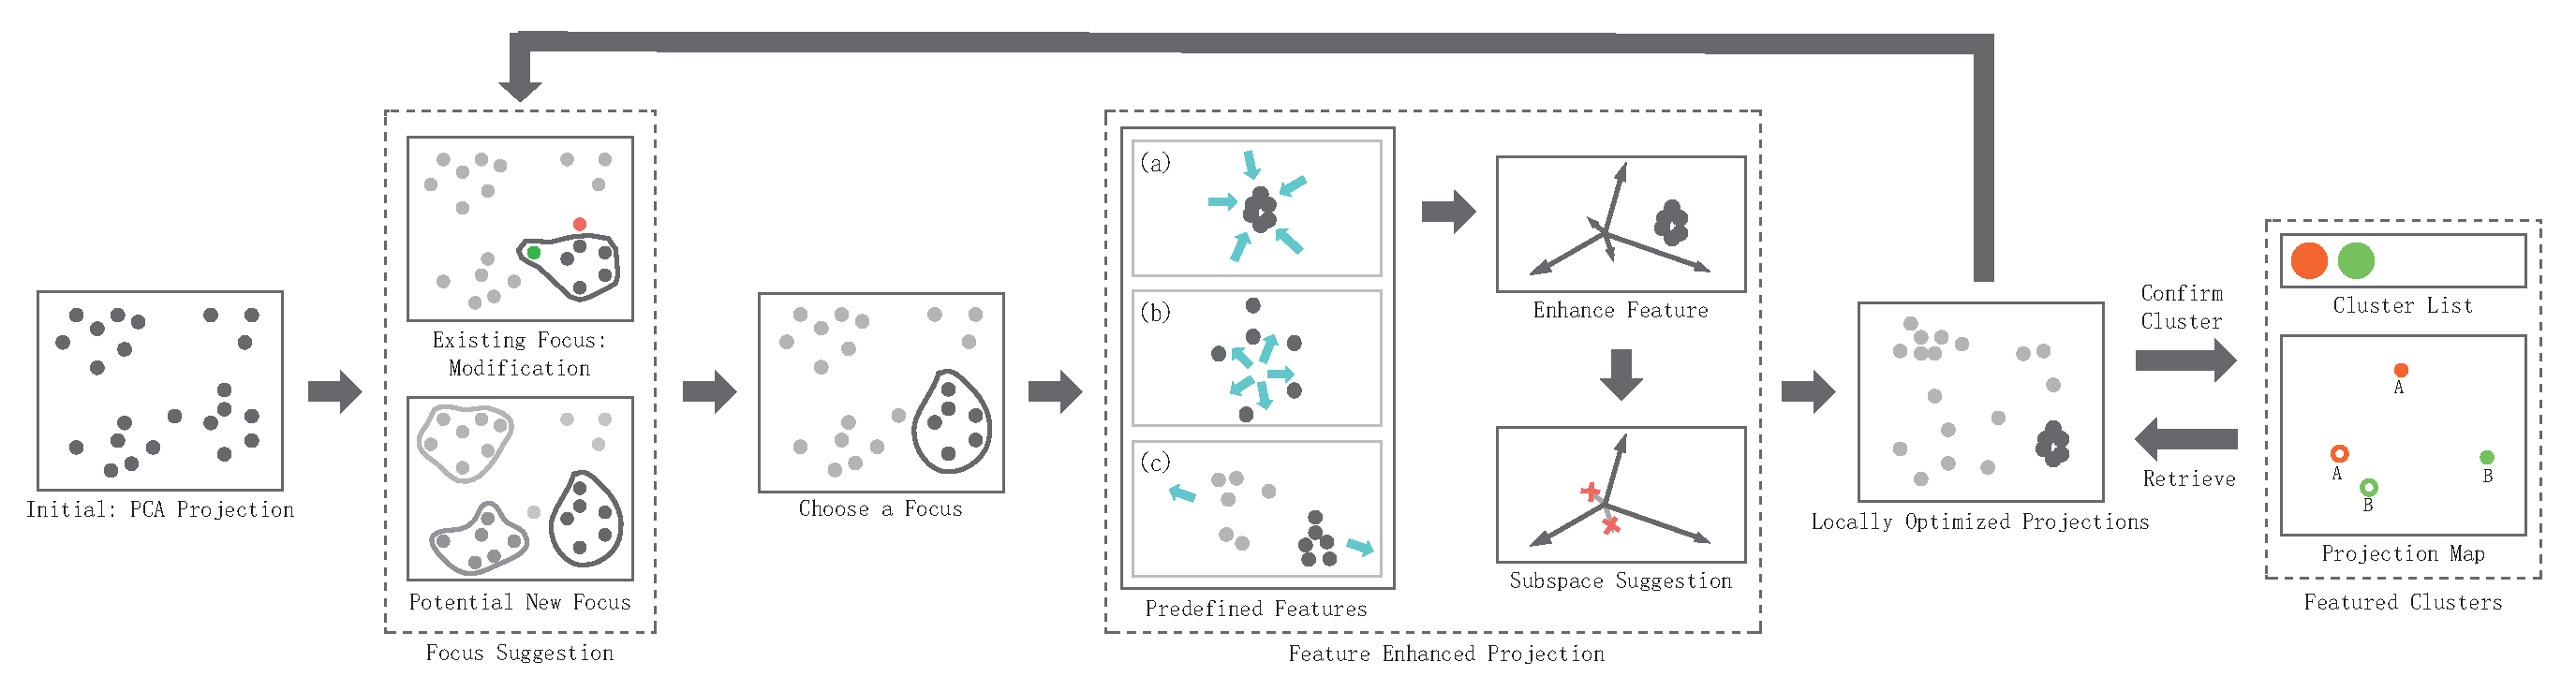
\includegraphics[width=1\linewidth]{images/Pipeline.eps}% 1\linewidth
  \caption{The overview of delivery system.}
\label{fig:workflow}
  \end{figure*}
  \fi

\subsection{Workflow}
Our method promotes an efficient high-dimensional data exploration, by facilitating distortion-free local analysis. It not only helps to maintain a faithful perception, but aims to enhance local features for better information mining. To be specific, the exploration contains four steps (see Figure~\ref{fig:workflow}):
\begin{enumerate}[Step. 1:]
 \item First, we present a globally optimized projection as an overview of the data. For the given projection, we help the user find a piece of interesting local data. Projection distortion and cluster suggestions are displayed to indicate potential outliers and clusters. The data chosen by user is called a \emph{focus}, meaning that it's the current focus in local analysis.
 \item After some focus is chosen, we find its most featured projections for a targeted analysis. By 'features', we refer to three kinds of local data relationships we defined. Projections are optimized to show these relationships with the least distortion. Based on the projection, we suggest a dimensional subspace that's most related to the feature. Its dimensions help to explain causes of the relationships.
 \item Since the focus is chosen in a projection, it could be a false cluster or missing some important pieces. We provide suggestions to help shape the focus into a more consistent and complete cluster. Whenever the focus is changed, the featured projections will also be updated. The process then returns to Step 2. This loop goes on until the user fully understands structures of the focus, and acquires a satisfactory cluster. After that, he can save the results and transfer his attention to another focus, returning to step 1.
 \item When some informative local data is found, the user can store it in the focus list for a further analysis. A 'projection map' is provided for featured projections of all focuses. It helps to compare different focuses, and navigate the high-dimensional exploration.
\end{enumerate}
The whole process is all about clarifying data relationships and figuring out the causes. Users never have to worry about configuring the projection. They are able to transfer seamlessly between different local analyses. In the next section, we'll introduce in detail how we support such exploration in each step.